\documentclass[12pt]{article}
\usepackage{scrextend}
\usepackage[utf8]{inputenc}
\usepackage[polish]{babel}
\usepackage[T1]{fontenc}%polskie znaki
\usepackage[utf8]{inputenc}%polskie znaki
\usepackage{geometry}
\usepackage{float}
\usepackage{enumitem}
\usepackage{hyperref}
\usepackage{graphicx}
\usepackage{tabulary}
\usepackage{etoc}
\usepackage[normalem]{ulem} 
\renewcommand{\baselinestretch}{1.5}
\graphicspath{ {img/} }
\newgeometry{lmargin=2cm, rmargin=2cm, tmargin=2cm, bmargin=2cm}
\usepackage{tikz}
\usepackage[bf]{caption}
\usepackage{setspace}
\usepackage{rotating}
\newcommand{\scenario}[5]{
  \subsection{#1}
  \begin{minipage}{\textwidth}
    \textbf{Cel:} #2 \\
    \textbf{WS:} #3 \\
    \textbf{WK:} #4 \\
    \textbf{Przebieg:}
    \begin{enumerate}
      \setlength\itemsep{0.0em}
      #5
    \end{enumerate}
  \end{minipage}
}
\hyphenation{include}
\hyphenation{extend}

\begin{document}

\begin{flushleft}
        Damian Koper, \textbf{241292} \\
        Łukasz Handschuh, \textbf{241402}
\end{flushleft}
\vspace{1cm}
{
    \centering
    {\Huge\scshape\bfseries Inżynieria oprogramowania - Etap 3 }\\
    \vspace{0.25cm}
    \Large\textbf{Dział ewidencji ludności} \\
    \vspace{0.25cm}
    \large Budowa diagramu czynności reprezentującego model
    biznesowy „świata rzeczywistego” na podstawie
    wykonanego opisu procesów biznesowych. Budowa
    diagramów czynności reprezentujących scenariusze
    wybranych przypadków użycia.\\
}

\section{PU Wyświetlanie wniosków}
\scenario
    {Wyświetlanie wniosków}
    {Wyświetlenie wymaganych wniosków.}
    {Inicjalizacja przez uruchomienie programu.}
    {Wyświetlenie wniosków.}
    {
        \item Należy wybrać wyświetlanie wniosków.
        \item Wszystkie wnioski przyporządkowane do danego urzędu zostają wyświetlone.
    }
\scenario
    {Zmiana kryterium wyświetlania wniosków}
    {Zawężenie poszukiwań wniosków.}
    {Musi zostać wywołany z \textit{Wyświetlanie wniosków}.}
    {Wyświetlenie tylko wniosków spełniających kryteria.}
    {
        \item Należy wprowadzić kryteria takie jak PESEL, imię i nazwisko.
        \item Wnioski spełniające podane kryteria są wyświetlane w formie tabeli.
    }

    \begin{sidewaysfigure}[!h]
        \centering
        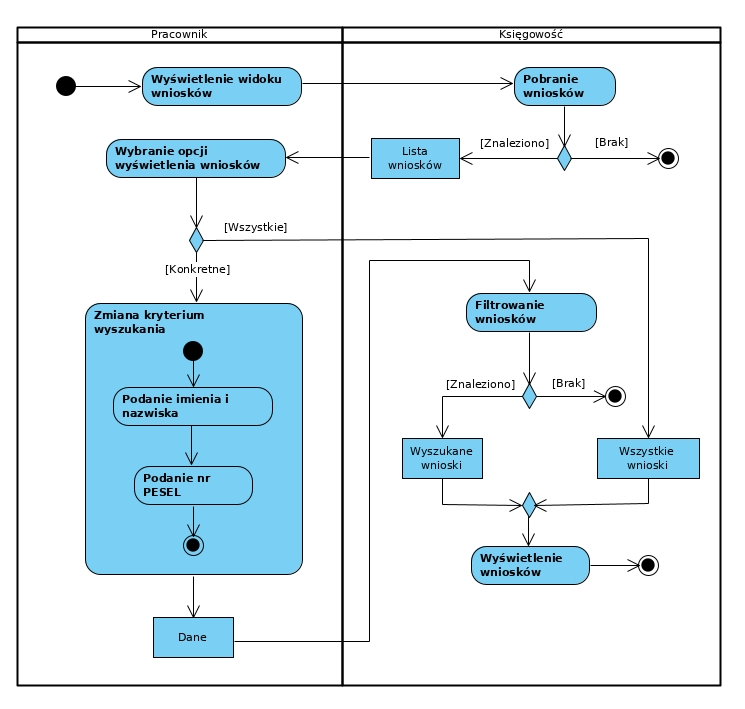
\includegraphics[
            keepaspectratio,
            width=\linewidth,
            height=\dimexpr\textheight-9\baselineskip
        ]{./../paragidm/export/PopulationRegistry_AD_2.jpg}
        \caption{PU Wyświetlanie wniosków - model biznesowy}
        \label{}
    \end{sidewaysfigure}

    \begin{sidewaysfigure}[!h]
        \centering
        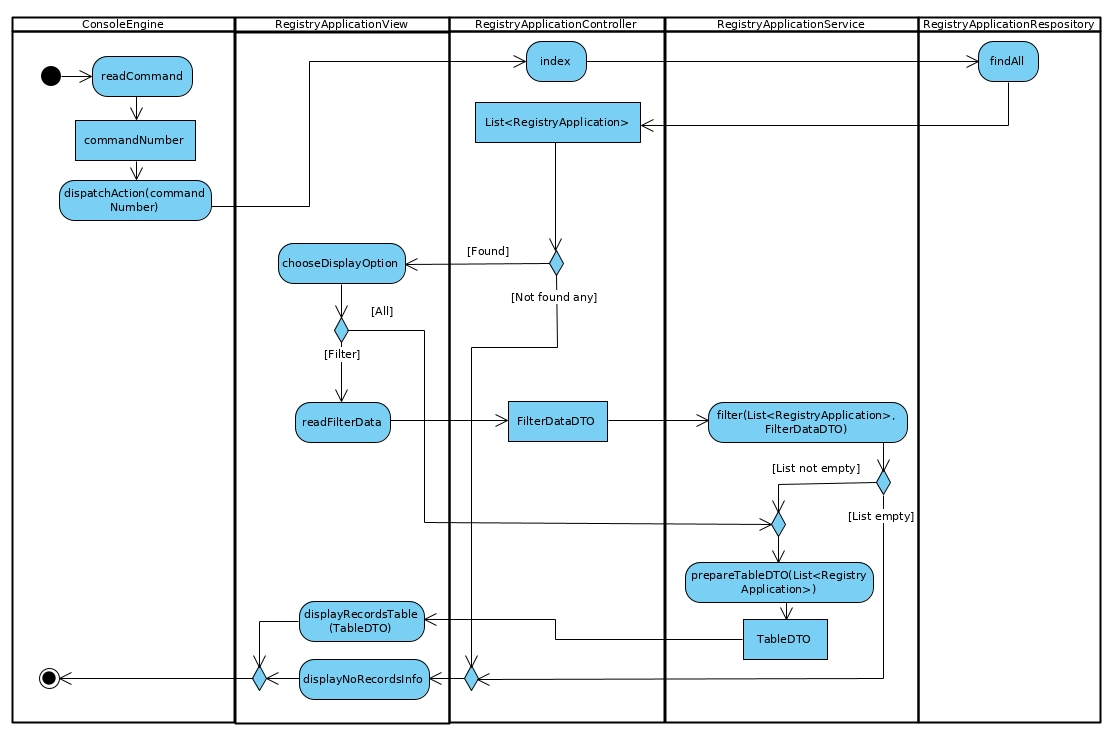
\includegraphics[
            keepaspectratio,
            width=\linewidth,
            height=\dimexpr\textheight-9\baselineskip
        ]{./../paragidm/export/PopulationRegistry_AD_2_1.jpg}
        \caption{PU Wyświetlanie wniosków}
        \label{}
    \end{sidewaysfigure}

\section{PU Edycja danych wniosku}

\scenario
    {Edycja danych wniosku}
    {Zmiana danych dotyczących wniosku.}
    {Inicjalizacja przez uruchomienie programu.}
    {Zaktualizowanie danych wniosku, lub wyświetlenie komunikatu o błędzie.}
    {
        \item Należy wpisać numer edytowanego wniosku.
        \item Jeśli wniosek nie został znaleziony wyświetlany jest komunikat o braku wniosku o wpisanym numerze.
        \item Należy wprowadzić nowe dane osobowe oraz nowe dane adresowe i zaktualizować status wniosku.
        \item Jeśli status zostanie zmieniony należy wywołać \textit{Zmiana statusu wniosku}
        \item Jeśli dane osobowe, lub dane adresowe zostaną zmienione należy wywołać \textit{Sprawdzanie poprawności danych}, które odbędzie się w systemie PESEL.
        \item Jeśli nowe dane okażą się prawidłowe wniosek jest aktualizowany i wyświetlany jest komunikat informujący o prawidłowej edycji, w przeciwnym razie użytkownik jest informowany o błędzie.
    }

\scenario
    {Zmiana statusu wniosku}
    {Odrzucenie, lub zaakceptowanie wniosku.}
    {Musi zostać wywołana z \textit{Edycja danych wniosku}.}
    {Wniosek zostaje odrzucony lub zaakceptowany.}
    {
        \item Należy zmienić status wniosku na odrzucony lub zaakceptowany.
        \item Jeśli wniosek został zaakceptowany należy wywołać \textit{Dodanie meldunku}.
    }

    \begin{sidewaysfigure}[!h]
        \centering
        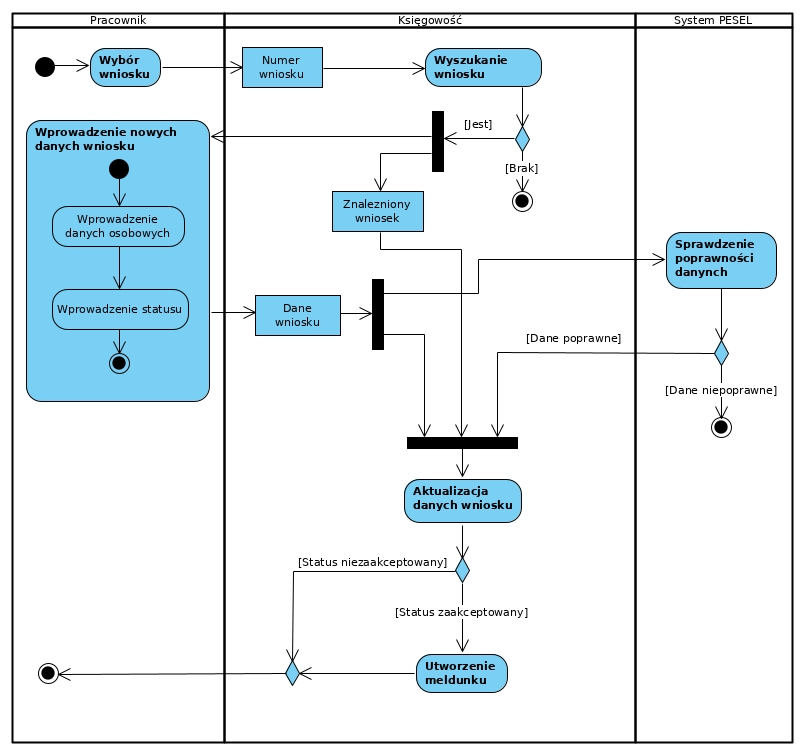
\includegraphics[
            keepaspectratio,
            width=\linewidth,
            height=\dimexpr\textheight-9\baselineskip
        ]{./../paragidm/export/PopulationRegistry_AD_1.jpg}
        \caption{PU Edycja danych wniosku - model biznesowy}
        \label{}
    \end{sidewaysfigure}

    \begin{sidewaysfigure}[!h]
        \centering
        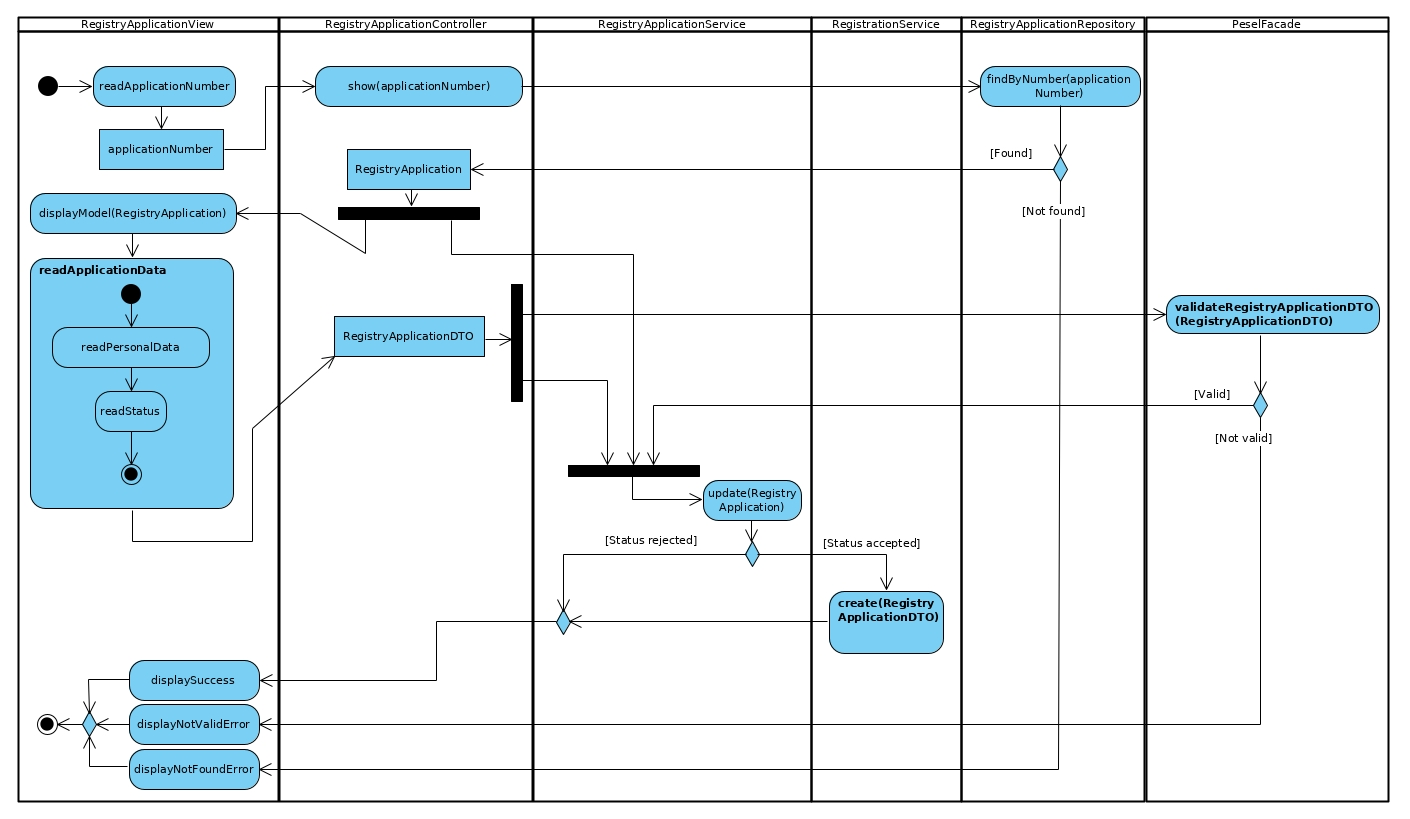
\includegraphics[
            keepaspectratio,
            width=\linewidth,
            height=\dimexpr\textheight-9\baselineskip
        ]{./../paragidm/export/PopulationRegistry_AD_1_1.jpg}
        \caption{PU Edycja danych wniosku}
        \label{}
    \end{sidewaysfigure}

\end{document}